% Gemini theme
% https://github.com/anishathalye/gemini

\documentclass[xelatex]{beamer}

% ====================
% Packages
% ====================

\usepackage[T1]{fontenc}
\usepackage{lmodern}
\usepackage[size=custom,width=120,height=72,scale=1.0]{beamerposter}
\usetheme{gemini}
\usecolortheme{uci}
\usepackage{graphicx}
\usepackage{booktabs}
\usepackage{tikz}
\usepackage{pgfplots}
\usepackage{amsmath}
\usepackage{algorithmic}

%\graphicspath{{/home/au/mkarikom/Lab/My\ Talks/NIPS/Poster/Image/}} %Setting the graphicspath 
\DeclareGraphicsExtensions{.pdf, .png, .jpg, .jpeg, .eps}

% ====================
% Lengths
% ====================

% If you have N columns, choose \sepwidth and \colwidth such that
% (N+1)*\sepwidth + N*\colwidth = \paperwidth
\newlength{\sepwidth}
\newlength{\colwidth}
\setlength{\sepwidth}{0.025\paperwidth}
\setlength{\colwidth}{0.3\paperwidth}

\newcommand{\separatorcolumn}{\begin{column}{\sepwidth}\end{column}}

% ====================
% Title
% ====================

\title{Learning Sparsely-Coupled Signaling Networks from Data}

\author{Matt Karikomi \inst{1} \inst{2} \and Qing Nie \inst{1} \inst{2}}

\institute[shortinst]{\inst{1} Deptartment of Mathematics, University of California, Irvine \samelineand \inst{2} The NSF-Simons Center for Multiscale Cell Fate}

% ====================
% Footer (optional)
% ====================

\footercontent{
  %\href{https://www.example.com}{https://www.example.com} \hfill
  NeurIPS 2019, Vancouver --- Learning Meaningful Representations of Life \#1 \hfill
  \href{mailto:mkarikom@uci.edu}{mkarikom@uci.edu}}
% (can be left out to remove footer)

% ====================
% Body
% ====================

\begin{document}

\addtobeamertemplate{headline}{}
{
%	\begin{tikzpicture}[remember picture,overlay]
%	\node [anchor=north west, inner sep=3cm] at ([xshift=-1.6cm,yshift=1.8cm]current page.north west)     {
\includegraphics[height=9cm]{Image/UCI_SEAL}};
%	\end{tikzpicture}
%
%	\begin{tikzpicture}[remember picture,overlay]
%	\node [anchor=north east, inner sep=3cm] at ([xshift=.7cm,yshift=.95cm]current page.north east)     {
\includegraphics[height=7.5cm]{Image/cmcf}};
%	\end{tikzpicture}
	
	\begin{tikzpicture}[remember picture,overlay]
	\node [anchor=north west, inner sep=3cm] at ([xshift=-0.5cm,yshift=2.2cm]current page.north west)     {
\includegraphics[height=7cm]{Image/UCI_SEAL}};
	\end{tikzpicture}
	
	\begin{tikzpicture}[remember picture,overlay]
	\node [anchor=north east, inner sep=3cm] at ([xshift=0cm,yshift=1.2cm]current page.north east)     {
\includegraphics[height=5.5cm]{Image/cmcf}};
	\end{tikzpicture}
}

\begin{frame}[t]
\begin{columns}[t]
\separatorcolumn

\begin{column}{\colwidth}

  \begin{block}{Juxtacrine Signaling via First-Neighbor Interactions}

    Lateral inhibition feedback networks form boundaries and repeating patterns by destabilizing symmetric expression of fate-genes in the embryo:

	\begin{figure}
		\centering
		\begin{minipage}{0.4\textwidth}
			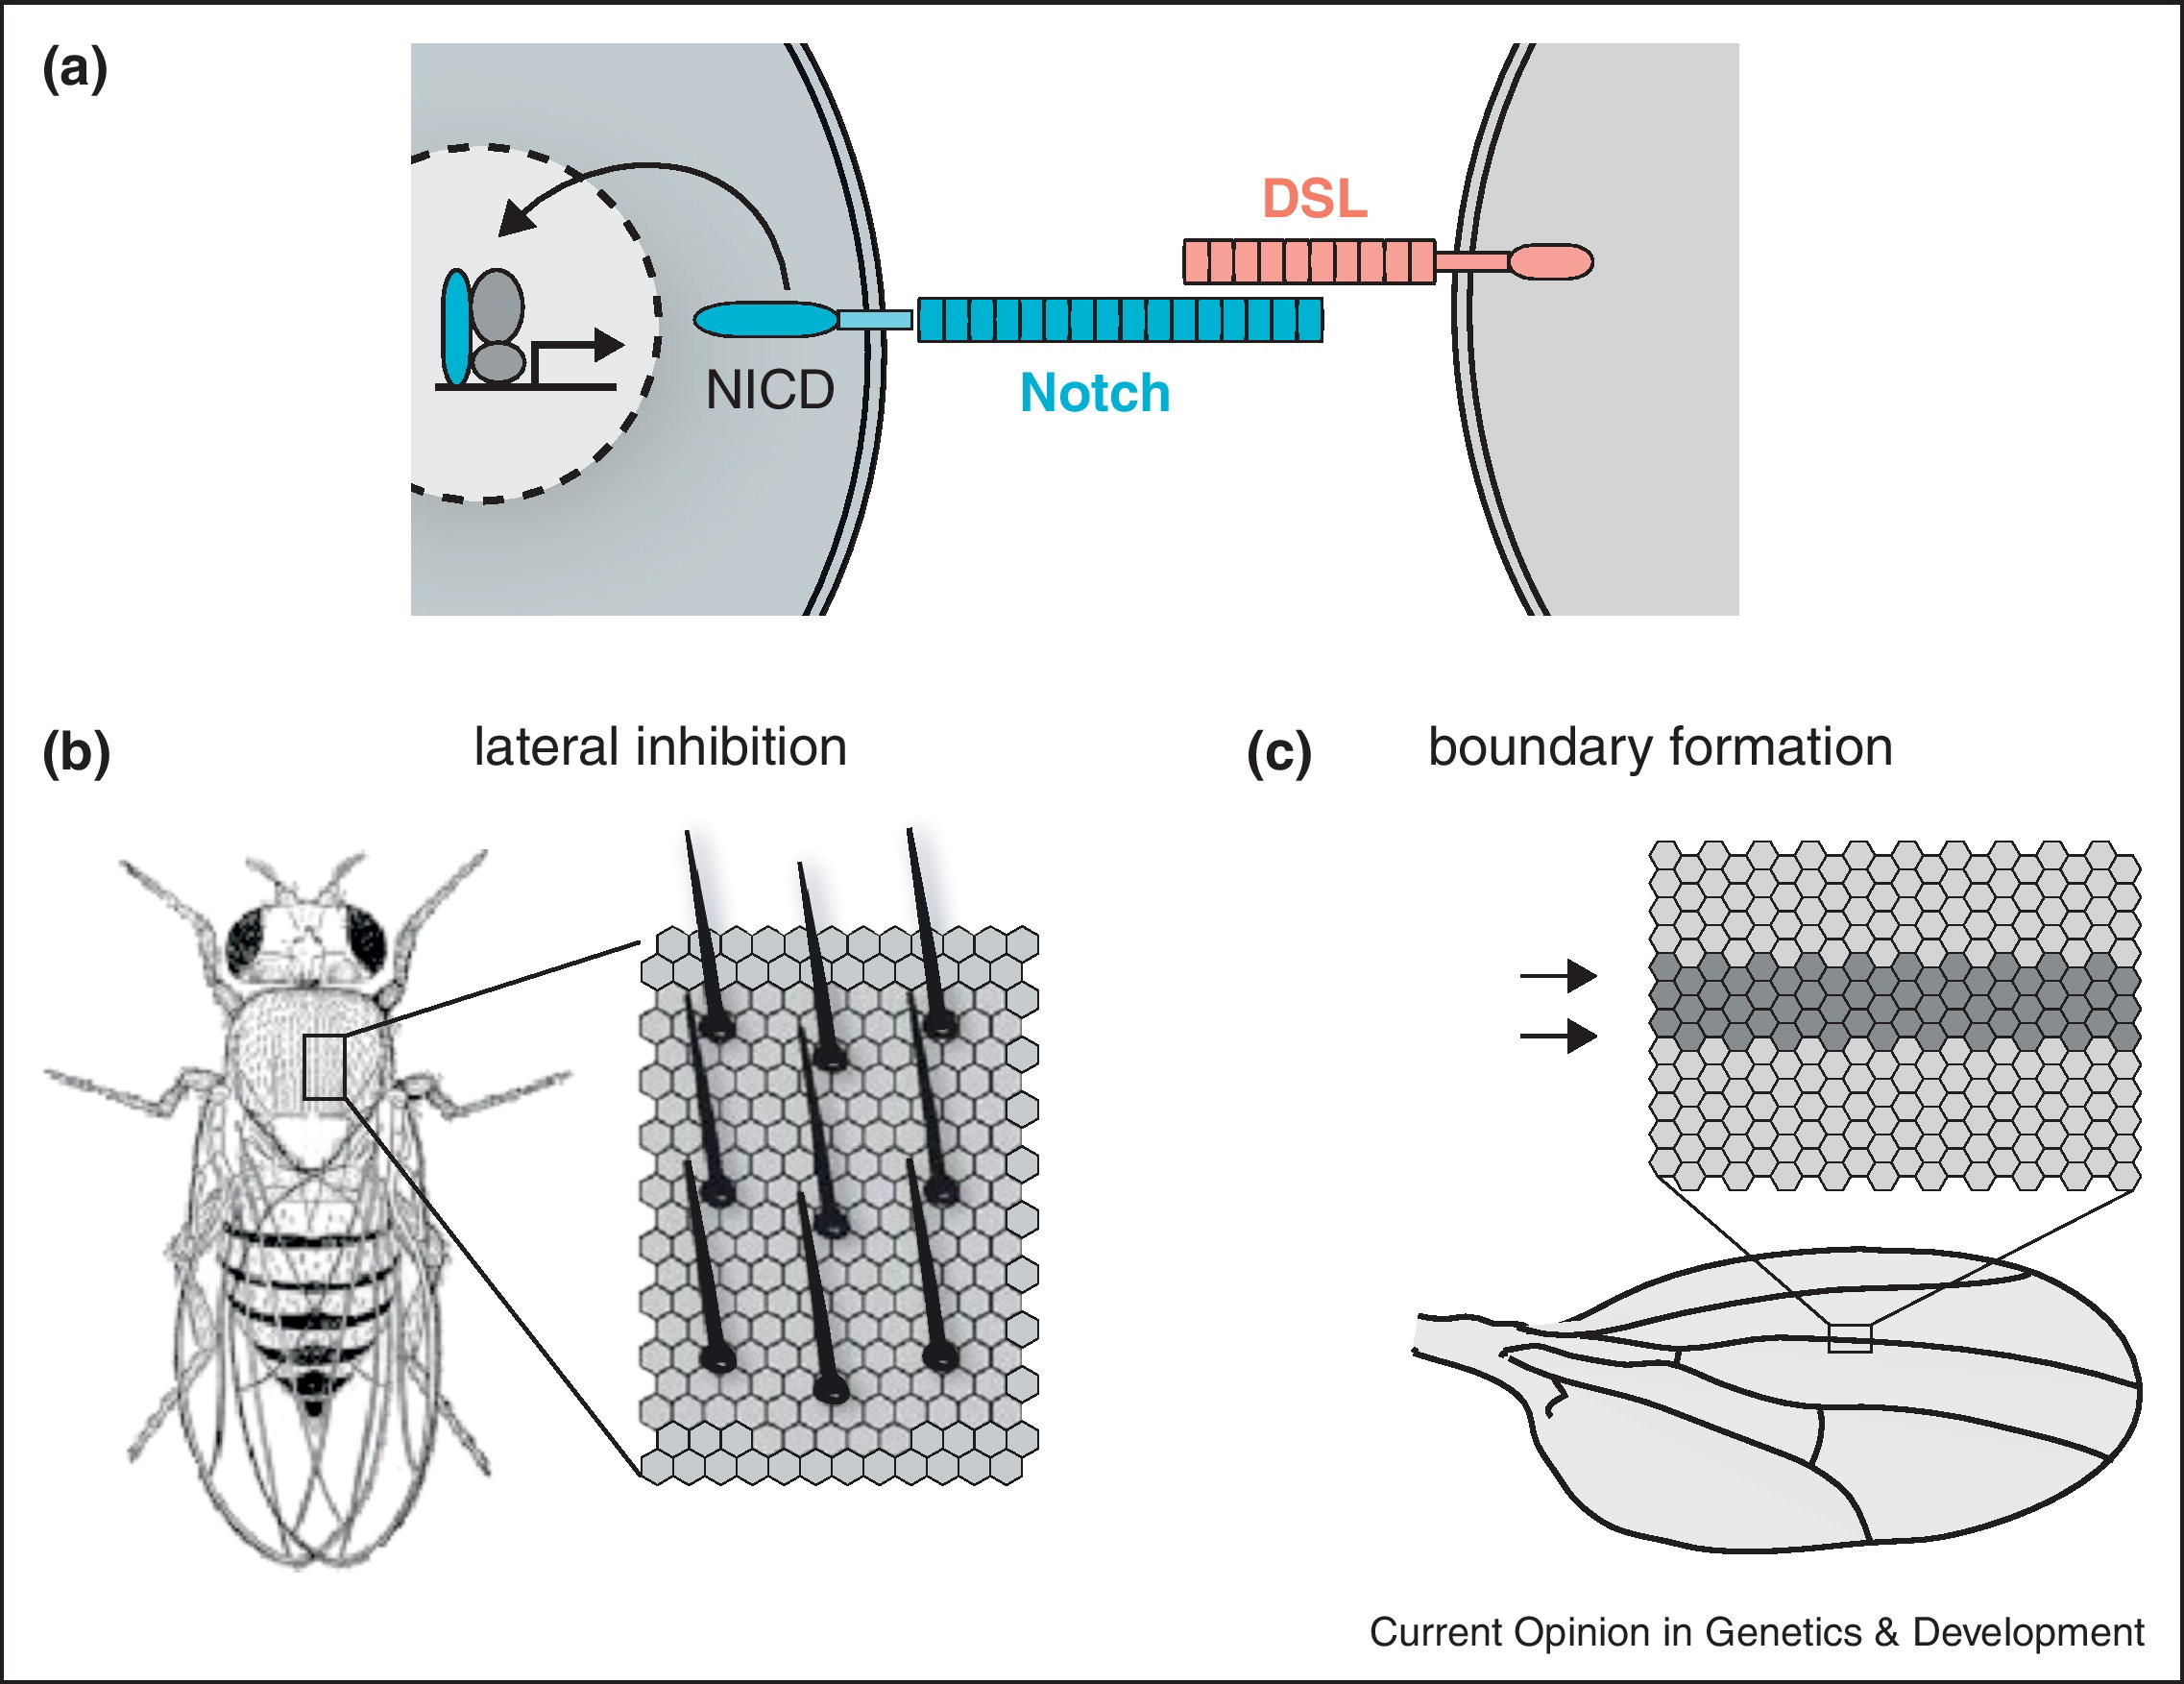
\includegraphics[scale=1.25]{Image/fly}
			\caption{Notch-Delta signaling controls patterning in neuronal lineages \cite{shaya_notch_2011}}
		\end{minipage}
	\hspace{2.5cm}
		\begin{minipage}{0.4\textwidth}
			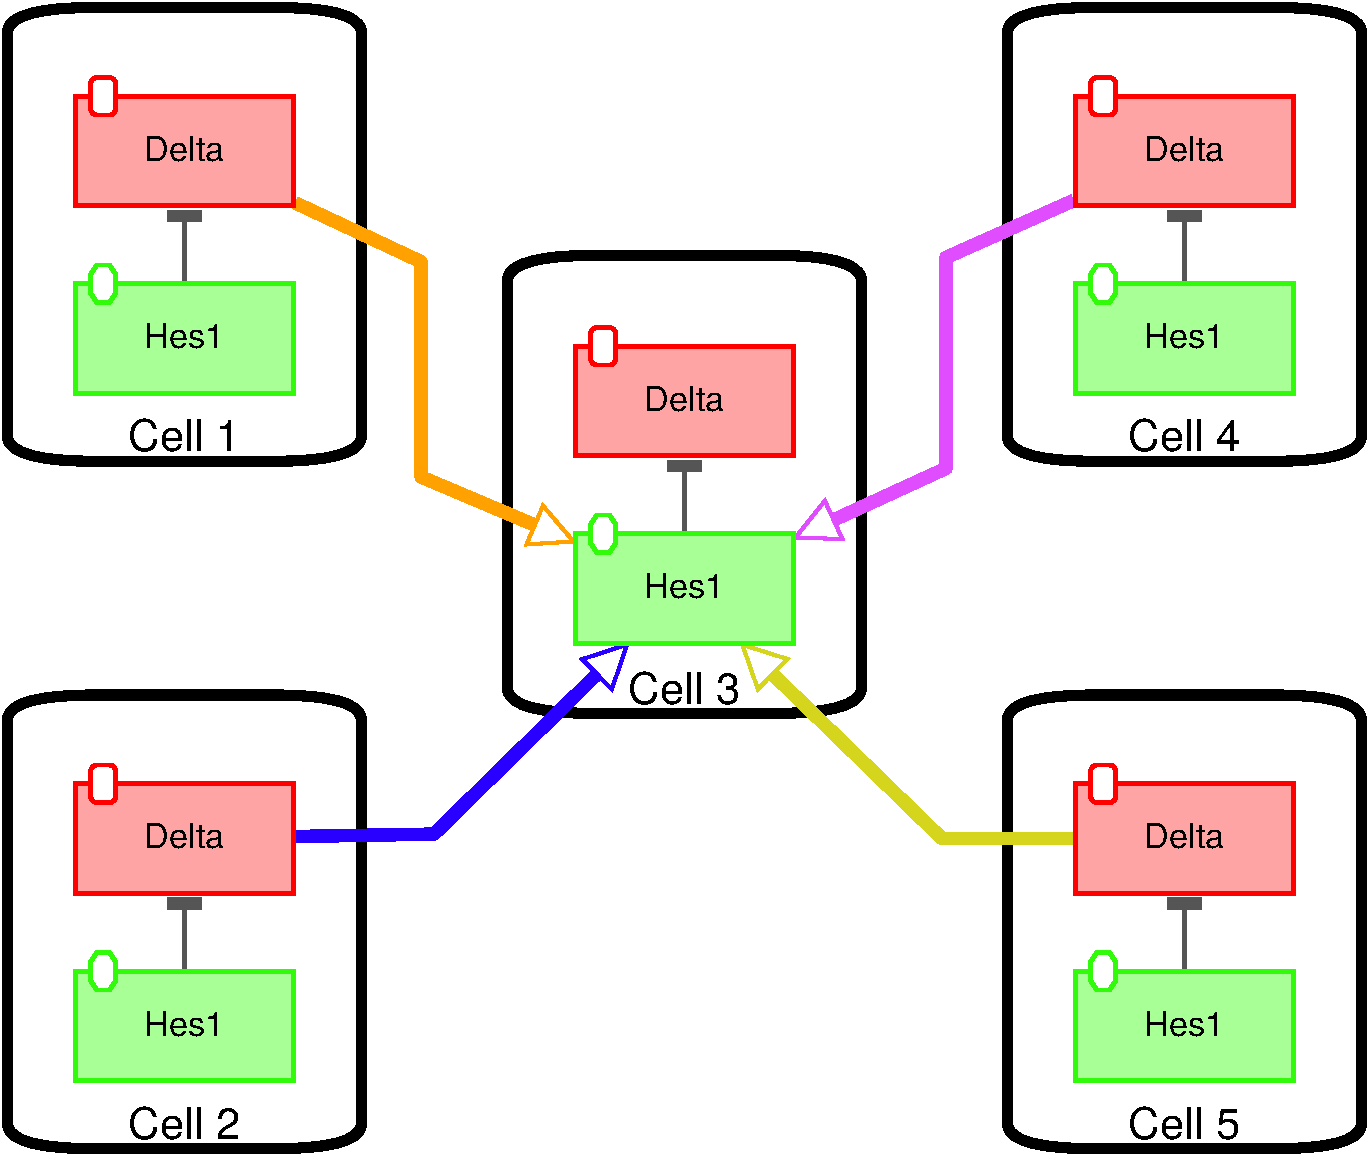
\includegraphics[scale=0.6]{Image/delta_LI_in}
			\caption{Delta from neighboring cells}
			\label{fig:li_in}
		\end{minipage}
	\end{figure}

	The network representation may be implicit (population model) or explicit (graph):
	\begin{itemize}
		\item \textbf{Non-destructive measurements} allow explicit reconstruction of the network by fitting dynamic models to longitudinal data
		\item \textbf{Destructive measurements} require assumptions about pattern geometry to convert the explicit model to population-level representation
		\item \textbf{Fully Coupled} Model requires a regularized fitting scheme.
		\item \textbf{Regularization} is based on the assumption that a fully connected network is unlikely (also impossible in the case of juxtacrine signaling) so a \textit{\textbf{sparse representation}} of the network is enforced via regularization.
	\end{itemize}
  \end{block}

\begin{alertblock}{Regularized Dictionary Learning}
	$\frac{\mathrm d \textit{H1}_i}{\mathrm dt} = F(\textit{H1}_i(t))$ is a linear combination of (trans) growth and (cis) inhibition.
	\begin{equation}\label{eq:state}
	\begin{split}
	F(\textit{H1}_i(t)) &= \text{the interpolant of } \textit{H1}_i(t)\\
	\Phi(\bm{d}(t)) &= \text{Hill-type transformations over Delta protein levels} \\
	\Psi(t) &=  \left [\Phi(\bm{d}(t)), \textit{H1}(t) \right] \\
	F(\textit{H1}_i(t)) &\approx \Psi(t) \bm{\beta_i} \\[1em]
	\end{split}
	\end{equation}
	Find the cross-validated Elastic Net estimate \cite{zou_regularization_2005} of $\beta$ for each cell.\\[1em]	
	\centering
	\begin{minipage}{0.7\textwidth}
		\begin{algorithmic}
			\STATE $Adj\gets zeros(|Cells|)$
			\FOR {cell $i$ in Cells} 
			\STATE $\bm{\hat{\beta_i}}_{CV} \gets \underset{\bm{\beta}}{\mathrm{argmin}} \left( \big|F(H1_i(t)) - \Psi(t)\bm{\beta} \big|^2 + \lambda_2 \big| \beta \big|^2 + \lambda_1 \big|\beta \big|_1  \right)$
			\FOR {cell $j$ in Cells}
			\IF {$sum[\bm{\hat{\beta_i}}_{CV}(1:j:end)] > 0$}
			\STATE $Adj(i,j) = 1$
			\ENDIF
			\ENDFOR
			\ENDFOR 
		\end{algorithmic}
	\end{minipage}
	\normalsize
\end{alertblock}

\end{column}

\separatorcolumn

\begin{column}{\colwidth}

\begin{alertblock}{Fate Determination: \\ Multistability of Notch Signal and Ligand Expression}

	\begin{figure}
		\centering
		\footnotesize
		\begin{minipage}{0.4\textwidth}
			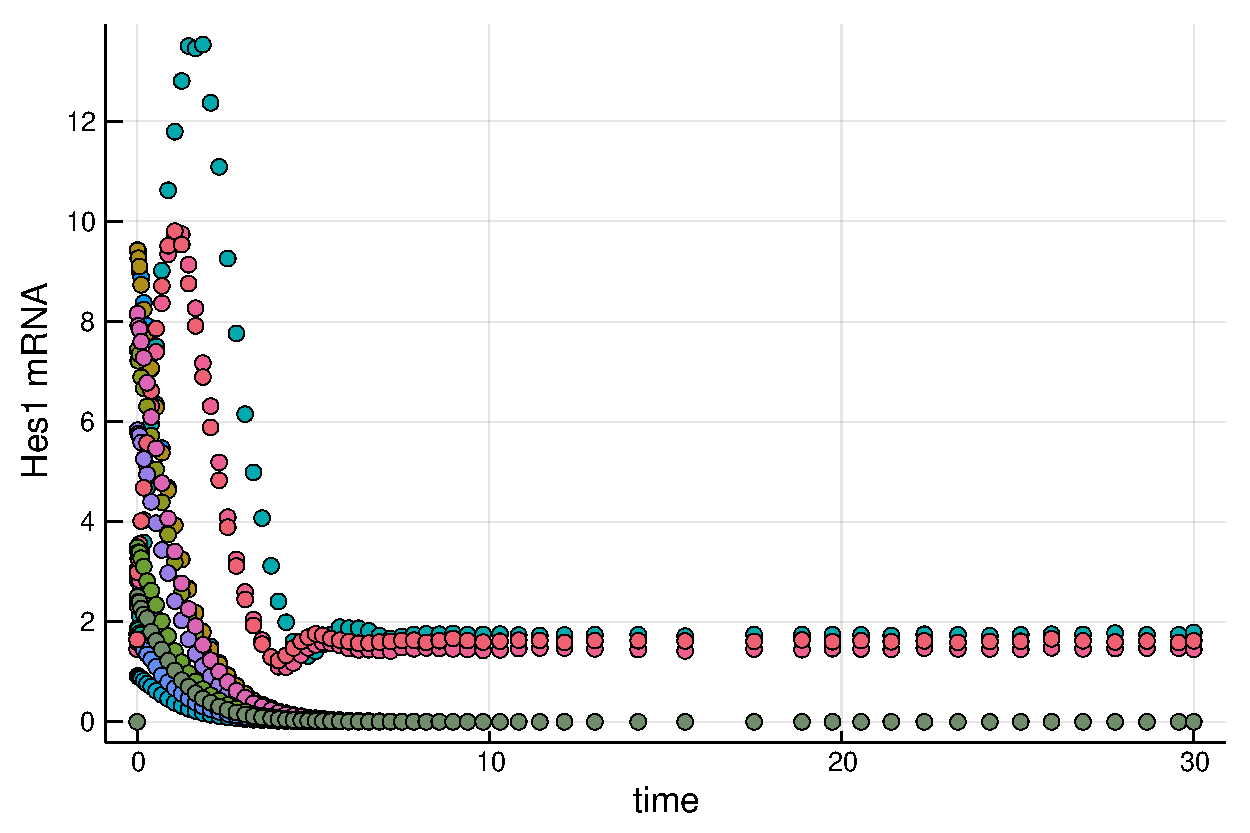
\includegraphics[scale=0.7]{Image/hes1_17cell_alpha-1_gamma.pdf}
			\caption{Notch signal}
		\end{minipage}
		\hspace{2.5cm}
		\begin{minipage}{0.4\textwidth}
			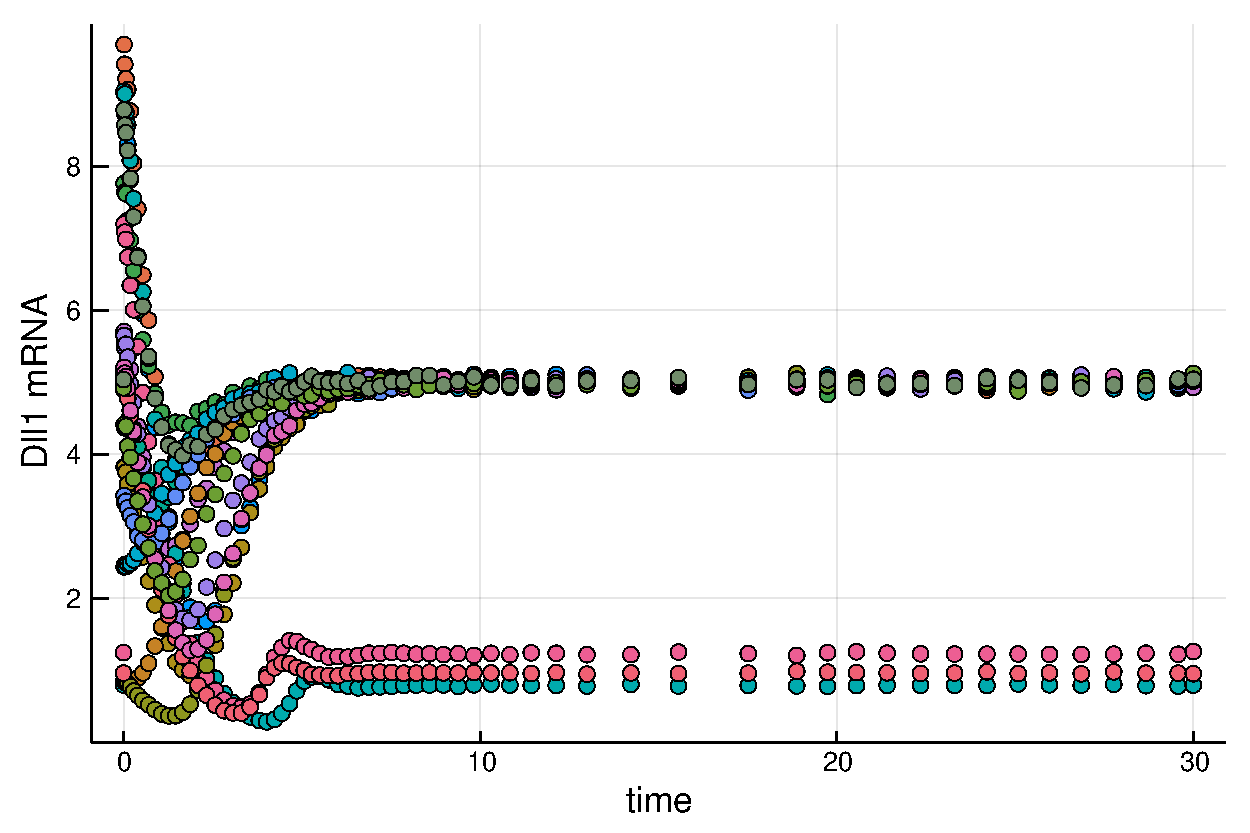
\includegraphics[scale=0.7]{Image/dll_17cell_alpha-1_gamma.pdf}
			\caption{Dll ligand expression}
			\label{fig:li_in}
		\end{minipage}
	\end{figure}
		\begin{figure}
	\centering
	\begin{minipage}{0.22\textwidth}
		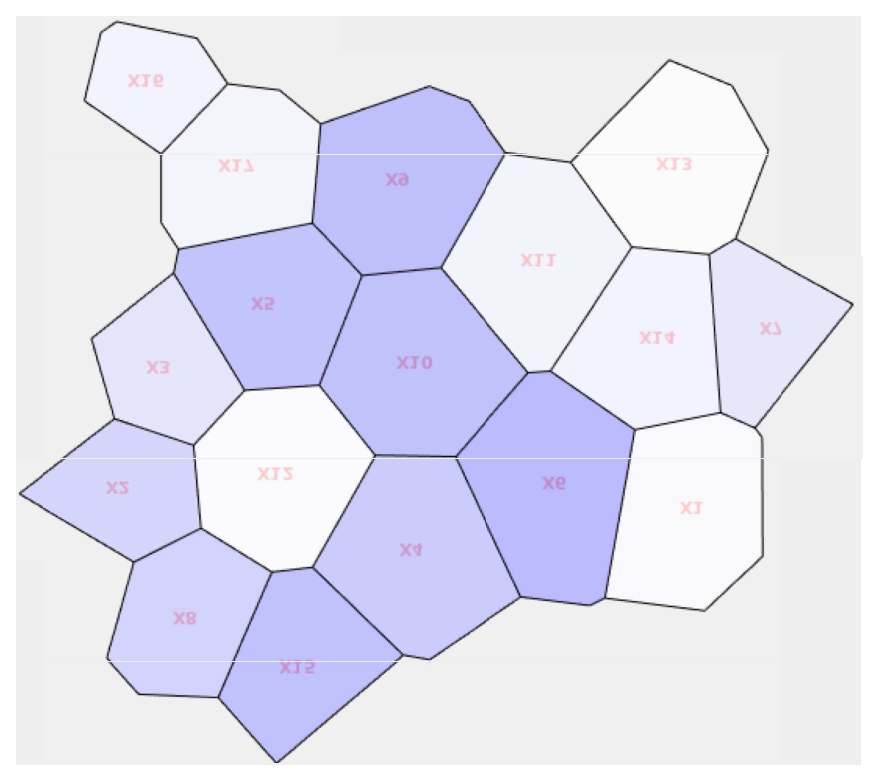
\includegraphics[height=7cm]{Image/Simulation_Delta_start}
	\end{minipage}
	\begin{minipage}{0.22\textwidth}
		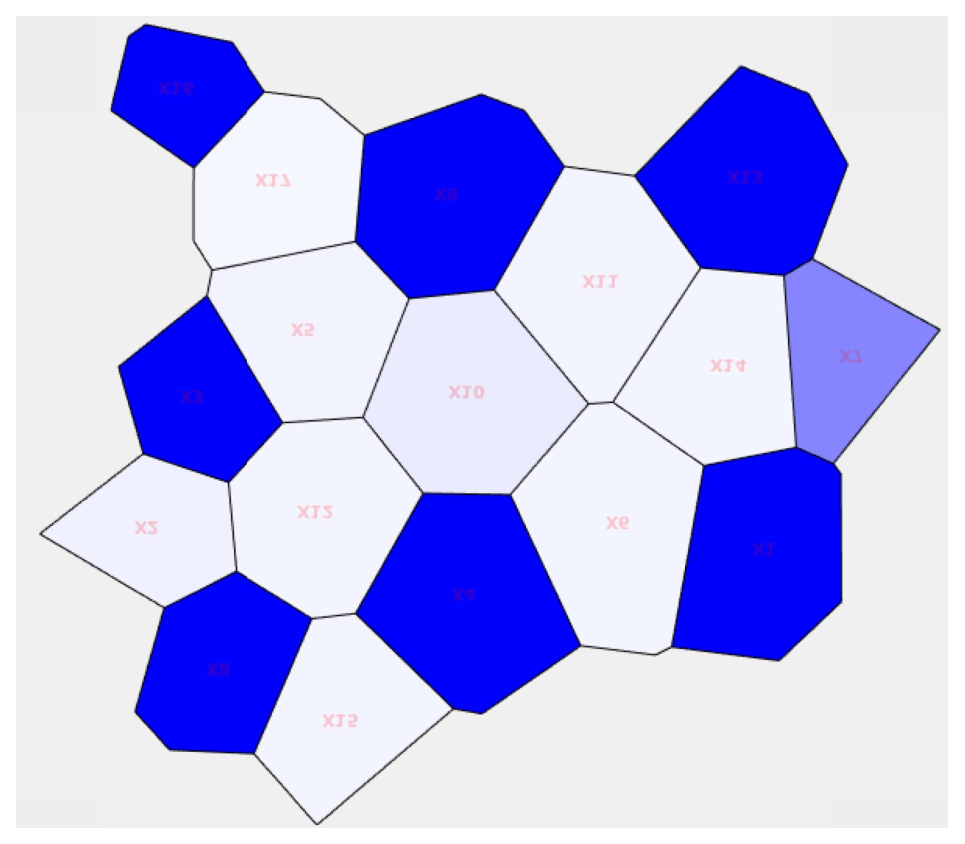
\includegraphics[height=7cm]{Image/Simulation_Delta_end}
	\end{minipage}
	\begin{minipage}{0.22\textwidth}
		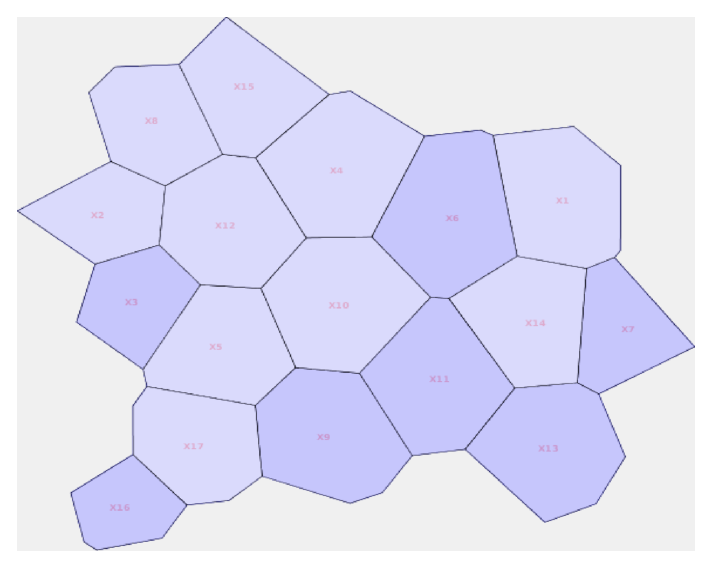
\includegraphics[height=7cm]{Image/Simulation_Hes1_start}
	\end{minipage}
	\begin{minipage}{0.22\textwidth}
		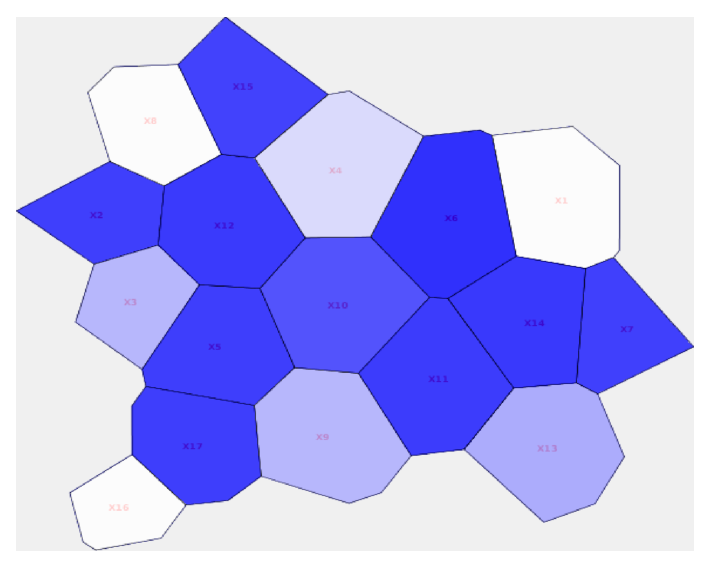
\includegraphics[height=7cm]{Image/Simulation_Hes1_end}
	\end{minipage}
	\caption{$\text{Delta}_{t=1}$, $\text{Delta}_{t=10}$,
		$\text{Hes1}_{t=1}$, $\text{Hes1}_{t=10}$}
\end{figure}

  \end{alertblock}

  \begin{alertblock}{Simulate Non-Destructive Time Series Measurement}
  	\begin{equation}\label{eq:delta}
  	\frac{\mathrm d d_i}{\mathrm dt} =
  	\nu \left(
  	\frac{\beta_{d,i}}{1 + \textit{H1}_i^h}
  	- d_i \right)
  	\end{equation}
  	\begin{equation}\label{eq:H1}
  	\frac{\mathrm d \textit{H1}_i}{\mathrm dt} =
  	\sum_{j \neq i}^{\Gamma(i)} \frac{\beta_{\textit{H1},i} \Delta d_j^m}{1 + \Delta d_j^m} - \textit{H1}_i
  	\end{equation}
  	\centering
  	\begin{tabular}{lll}
  		\toprule
  		Symbol & Description & Value \\
  		\midrule
  		$d_i$ & Delta protein &\\
  		$\textit{H1}_i$ & Hes1 protein &\\
  		$\textit{H1}^{obs}_i$ & Hes1 protein, noisy observation: $\mathcal{N}\left(\gamma \textit{H1}_i(t),0.1 \right)$ &\\
  		$\gamma$ & scaling for Gaussian noise on $\textit{H1}^{obs}_i$ & 0.01-0.1\\
  		$d_i(0), \textit{H1}_i(0)$ & randomly perturbed initial state & \\
  		$\beta_{d,i}$ & intrinsic Delta ligand production & 5\\
  		$\beta_{\textit{H1},i}$ & trans-activation strength & 20 \\
  		$\Delta$ & scaled shared cell membrane for unit grid tesselation & 0-1 \\
  		$m$,$h$ & activation and repression cooperativity & 3, 3\\
  		$\nu$ & timescale ratio: repressor/ligand dynamics & 1\\
  		$t$ & unitless time & 1:30 (model fitted on 1:15)\\
  		$\Gamma(i)$ & neighbors of cell $i$ &\\
  		\bottomrule
  	\end{tabular}
  	\normalsize
  \end{alertblock}

\end{column}

\separatorcolumn

\begin{column}{\colwidth}

  \begin{block}{Accuracy of the Explicit Solution}
	\begin{figure}
	\centering
	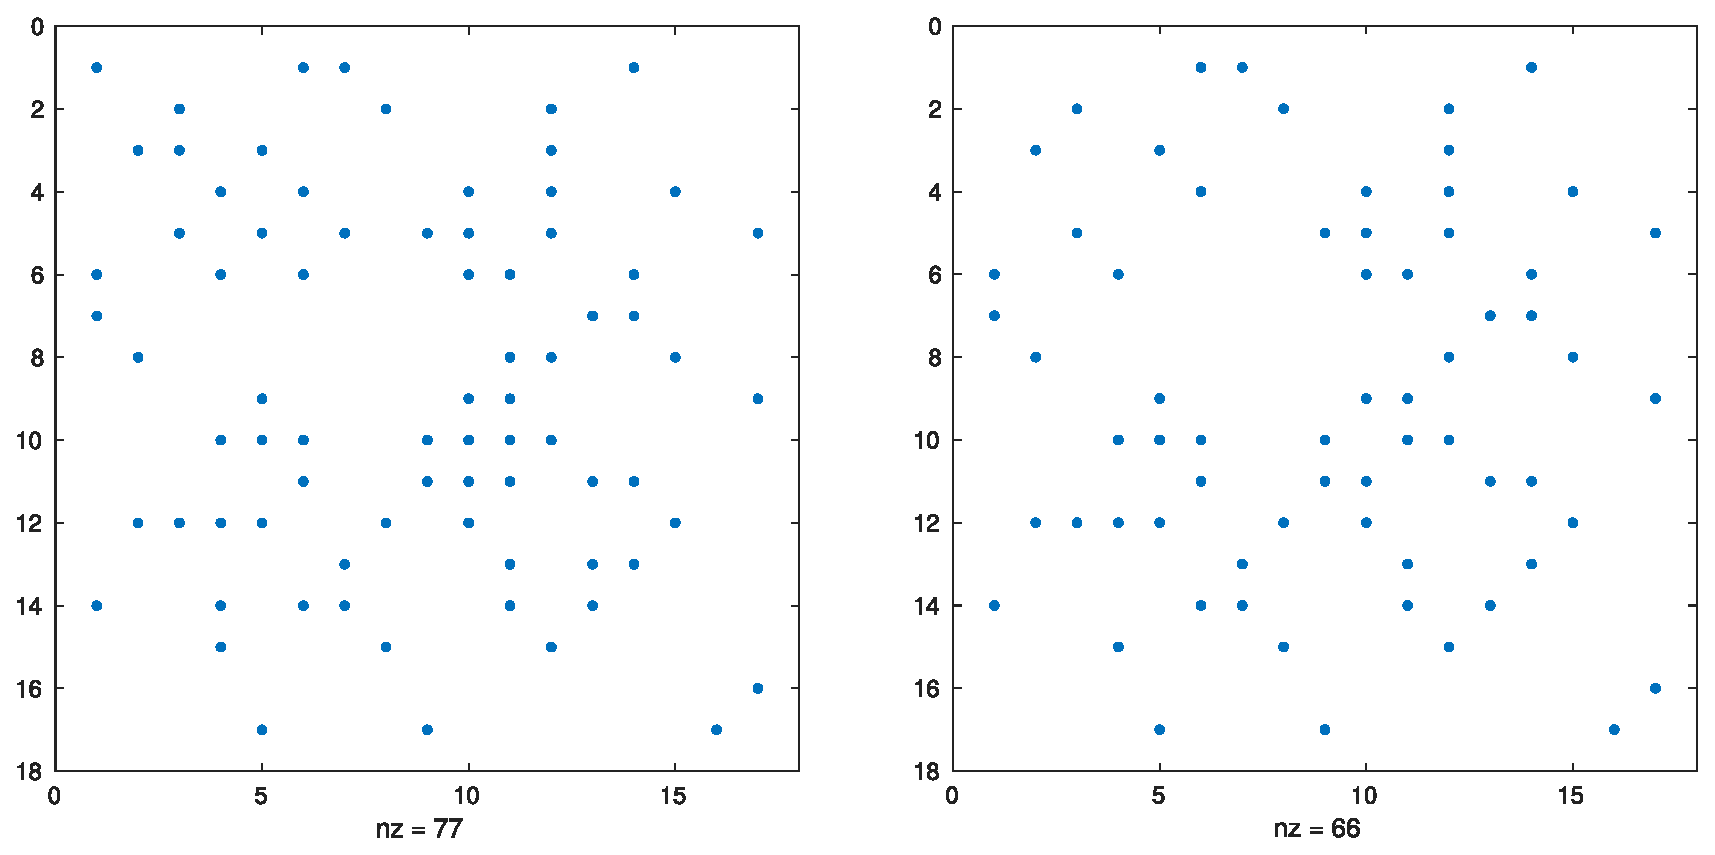
\includegraphics[width=\textwidth]{Image/adjfig}
	\caption{True adjacency vs. Estimated adjacency ($\alpha = 1, \gamma = 0.01$)}
	\label{fig:li_in}.
	\end{figure}
	\begin{figure}
		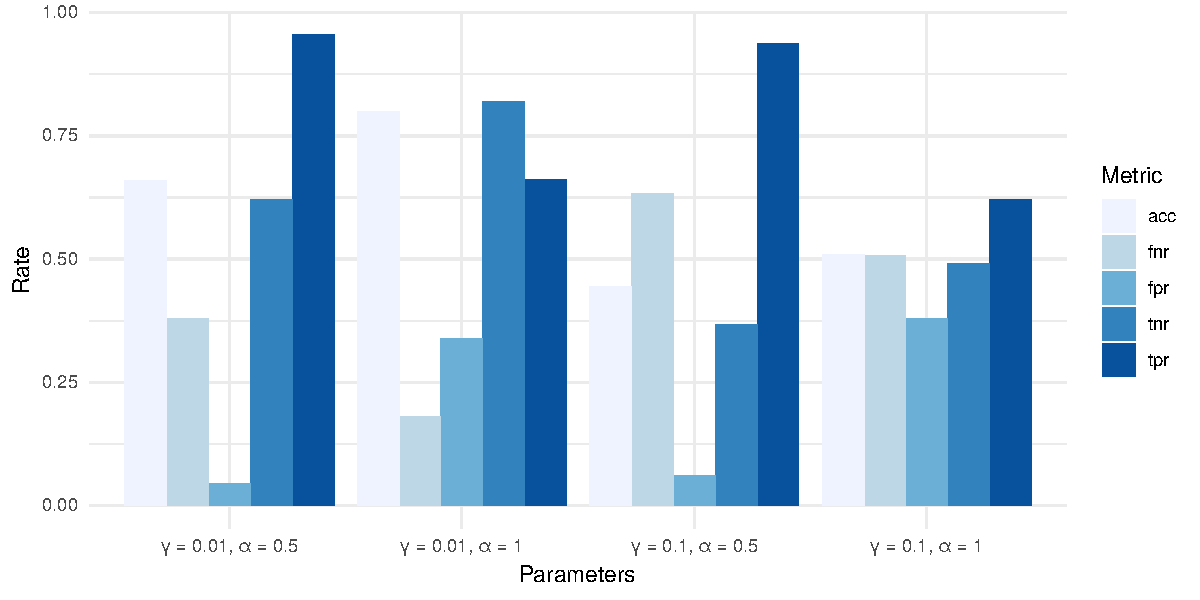
\includegraphics[width=0.8\textwidth]{Image/perf}
		\caption{Classification accuracy for $\Psi(d(t)) = \left[ \textit{H1}(t), \frac{\bm{d}^3}{1 + \bm{d}^ 3} , \frac{\bm{d}^4}{1 + \bm{d}^ 4}\right]$}
	\end{figure}
  \end{block}

  \begin{block}{References}

    \nocite{*}
    \footnotesize{\bibliographystyle{plain}\bibliography{poster}}

  \end{block}

\end{column}

\separatorcolumn
\end{columns}
\end{frame}
\end{document}
